%\documentclass{../_combined/fcg-book}
\chapter{Perception}
Our minds deceive us. Intuitively we feel we see very clearly and 
unambiguously the objects in our environment and are able 
to categorize objects or actions unequivocally in terms of 
perceptually grounded distinctions. For example, when 
I look out of the office window at the inner 
courtyard garden, I can clearly see the plants, trees
and birds, as well as the walls, windows, and doors of 
the surrounding buildings. I can categorize their 
colours, sizes, and shapes and determine whether the 
leaves of the trees are moving with the wind. Because of 
this categorisation I can describe to another person what 
I see. 

A categorisation and conceptualisation
of reality is fundamentally based on sensors which output 
signals that directly 
reflect, in an analog and partially unreliable way, physical
properties of the environment. For visual perception, 
human beings have photosensors in the eye which correlate 
with the amount of light, i.e. the amount of 
photons, falling on the sensor. The more photons, the stronger
the sensor signal. But, a photosensor, or a matrix of 
such sensors as in the human
retina, does not tell anything more than what the light
intensity is at a tiny spot of the image captured
by the eye. There is no obvious straightforward
procedure that groups the spots 
into coherent patches.
When you implement and tries out different segmentation procedures
on real world images, you quickly find that each procedure
generates a multitude of possibilities instead of a clear 
segmentation. Even if
coherent segments are detected, there is the problem of what 
features of the scene are going to be used for further
conceptualisation. A very large, open-ended
set of possible feature detectors can be
imagined. The quality and reliability of their
output depends on the scene being processed, and is in any 
case strongly context-dependent. 

So we find that the world does not present itself neatly segmented, 
processed, and categorized. There is an enormous 
gap between the symbolic world of objects and categories
and the subsymbolic world of analog sensing. 
The brain somehow performs a vast amount of processing
to fill this gap, without us being in the least aware of it. 
This processing takes place in parallel. Many different
segmentation procedures and feature detectors 
operate concurrently on streams of consecutive images, 
generating hypotheses that become stronger if they are
confirmed by additional evidence, or weaker if 
they do not fit into a larger picture. We are only 
aware of the final result and therefore have no 
intuition of what is really going on, except
in rare and pathological circumstances. 
Rather than viewing perception as a straight-forward step-by-step
transformation of the raw sensory data into a segmented
picture, it is better to think of the whole process
as a boiling soup with thousands of hypotheses taking
shape, some of them floating like bubbles up to the surface. Constraints
and expectations flow down from the top so that the maximum 
amount of available information is used to construct the 
coherent segmented picture of reality we consciously experience. 

The objective of this chapter is to examine this 
process in sufficient detail to move forward with the main
topic of our investigations, namely language and meaning. My 
aim is not to delve into the full complexity of the 
visual system, because this would lead us too far 
astray of the main topic, but to have a sufficiently 
rich source of features so that conceptualisation and 
language communication can be studied. 

\section{What sensors sense}

Sensors and actuators are the interfaces between the physical
world and the internal world. \is{sensors} \is{actuators} They are 
dedicated hard-wired components and grow in biological 
systems strongly influenced by genetics and environmental inputs.\footnote{Possible 
biological implementations of the various 
sensors and sensory processes discussed in this chapter 
can be found in \cite{Churchland:1992}. The 
nature and neurophysiological implementation of visual
processes are discussed in detail in \cite{Zeki:1993}.}

A sensor transduces external physical 
states into internal states. For example, a touch sensor, of which 
there are hundreds of thousands all over the human body, 
transduces mechanical energy into neural signals. Other sensors
respond to the intensity of certain sectors of the wave spectrum. 
Ears respond to audible waves. Photoreceptors in the eye
respond to visible light waves. 
The body also has a large number of
biochemical sensors responsive to internal 
chemical states so that we can feel the hunger in our stomach for example. 
In addition to sensors, bodies carry 
actuators, which transduce internal states into mechanical 
energy and thus make it possible to perform actions in 
the world. Actuators receive continuous signal streams and modulate
their activity based on these signals. 

\subsection{Artificial Sensors and Actuators}

Analogs of biological sensors can be artificially recreated to give
robots sensory capabilities. Something similar to 
a touch sensor can be created using a contact switch 
that passes current when closed. A microphone has 
a functionality similar to the ear. 
A digital camera can be used to recreate the functionality of an eye; 
it records the light intensity of millions of small rectangles of 
the image, known as pixels, just like the retina. The set of 
all pixels is usually called an image map. Digital
colour cameras provide three information elements for 
every pixel: the amount of red, 
green and blue of each pixel (RGB). We 
can build sonar sensors responding
to low frequency waves, just like the ones bats use 
for navigation, or infrared sensors which are useful 
for obstacle avoidance because 
the amount of infrared light emitted and captured back
by the sensor correlates with distance to objects. 

A sensor should never be seen as measuring accurately 
an abstract property of reality. For example, an infrared sensor 
does not measure the distance to an obstacle. The infrared
reflection depends not only on distance but also
on the reflection properties 
of the object and on the amount of background infrared 
in the environment, thus distance must be inferred and projected onto
reality. Similarly, the colour receptors do not really measure
colour. They respond to reflections within segments of the wavelength spectrum 
but this reflection is again determined by many factors: how much and what kind of 
light falls on the object, and how the object reflects the light depending which varies 
with the position of the object. So colour is again a more abstract notion that needs to be 
reconstructed and projected on the image based on complex processing. 

The Talking Heads use vision as the main source of
sensory information because most of the perceptually 
grounded concepts used in language derive from visual
sensing. The only actuator (apart from the speech 
synthesiser which I will not discuss in detail) 
is a pan/tilt motor for turning the head up and down 
or left and right. 

\subsection{Natural sensing}

It is technically possible to build all sorts of 
sensors and actuators that have little to do with
human capabilities. But clearly, human-like categories and languages 
that are similar to human categories and languages will only 
emerge if the sensors and actuators are at least to some degree similar to those
of humans. This is not always technologically 
possible and when it is, it often 
requires non-trivial transformations of artificial 
sensor data. The Talking Heads use digital cameras 
as their main sensory source. These cameras give output 
in RGB (red, green, blue intensities) because this 
is the standard in current computer 
technology. But human vision operates
on four quite different channels: the two chromatic 
opponent channels which provide a value on the 
yellow-blue and red-green dimensions, an achromatic 
channel which holds the brightness or light 
intensity, and a saturation channel which reflects the 
degree of saturation or purity of a colour. These 
channels can be reconstructed from RGB by a complex 
transformation.\footnote{
There is a vast literature on colour perception from 
different points of view (physics, psychology, 
neurophysiology, linguistics). A representative sample 
is contained in \cite{Byrne:1997}. 
In some of the experiments described later, the RGB values
are converted to the CIE XYZ colour coding and from 
that to the opponent channels. 
These algorithms have been implemented by Michael
Pollitis. See: \cite{Kaiser:1996}. 
}

\subsection{Behaviors}

Although language requires that the image is 
segmented and categorized, a lot can already
be done with raw or lightly processed sensory data
by dynamically coupling them to signals 
controlling the actuators. The neural abilities
of many simple animals probably do not get much further
than this and it already has turned
out to be a good way to construct the basic behavioral
layers of robots that have to operate autonomously 
in a real-world environment in real time. 

For example, suppose we want a robot of the sort seen 
in \figref{f:plate3} to move towards a light source. As originally 
suggested by the cybernetician Valentino Braitenberg,
\cite{Braitenberg:1984}. 
we can do this by mounting two simple light sensors 
to the left and right of the body and by implementing a 
direct dynamical coupling between the output of the light
sensors and the motors. The coupling is such that when
the sensed left light is stronger than the sensed right
light, the motor attached
to the left wheel is slightly decreased and the right
motor slightly increased, so that the robot veers to the left. 
When the right light is stronger, the right motor is 
increased and the left motor decreased, so that the 
robot veers to the right. When these two dynamical 
couplings are put in place together with a
forward movement, a zig-zag behavior emerges which
brings the robot to the light source. \is{behaviors}

Basic behaviors can be put together to form 
more complex behaviors.\footnote{A representative sample of experiments in this 
direction is reported in: \cite{Steels:1996}. See 
also: \cite{Arkin:1998}.}
\figref{phototaxis} 
shows a recording of the internal states of the robot
in \figref{f:plate3} as it is performing 
phototaxis towards a light source, using two simple
light sensors, and touch-based obstacle avoidance
behavior.  When the robot strikes the box housing 
the light, it moves back in a kind of reflex behavior
triggered by the touch sensors mounted at the front. 
The $LeftLight$ and 
$RightLight$ sensory channels and the $LeftMotorSpeed$ 
and $RightMotorSpeed$ are shown 
in \figref{phototaxis}. When the robot strikes
the obstacle housing the light, its left and right
motor is pulled down to a negative value so that 
it moves backwards. Then the robot zig-zags to the 
light source until it hits the obstacle again. 
\begin{figure}[htbp]
  \centerline{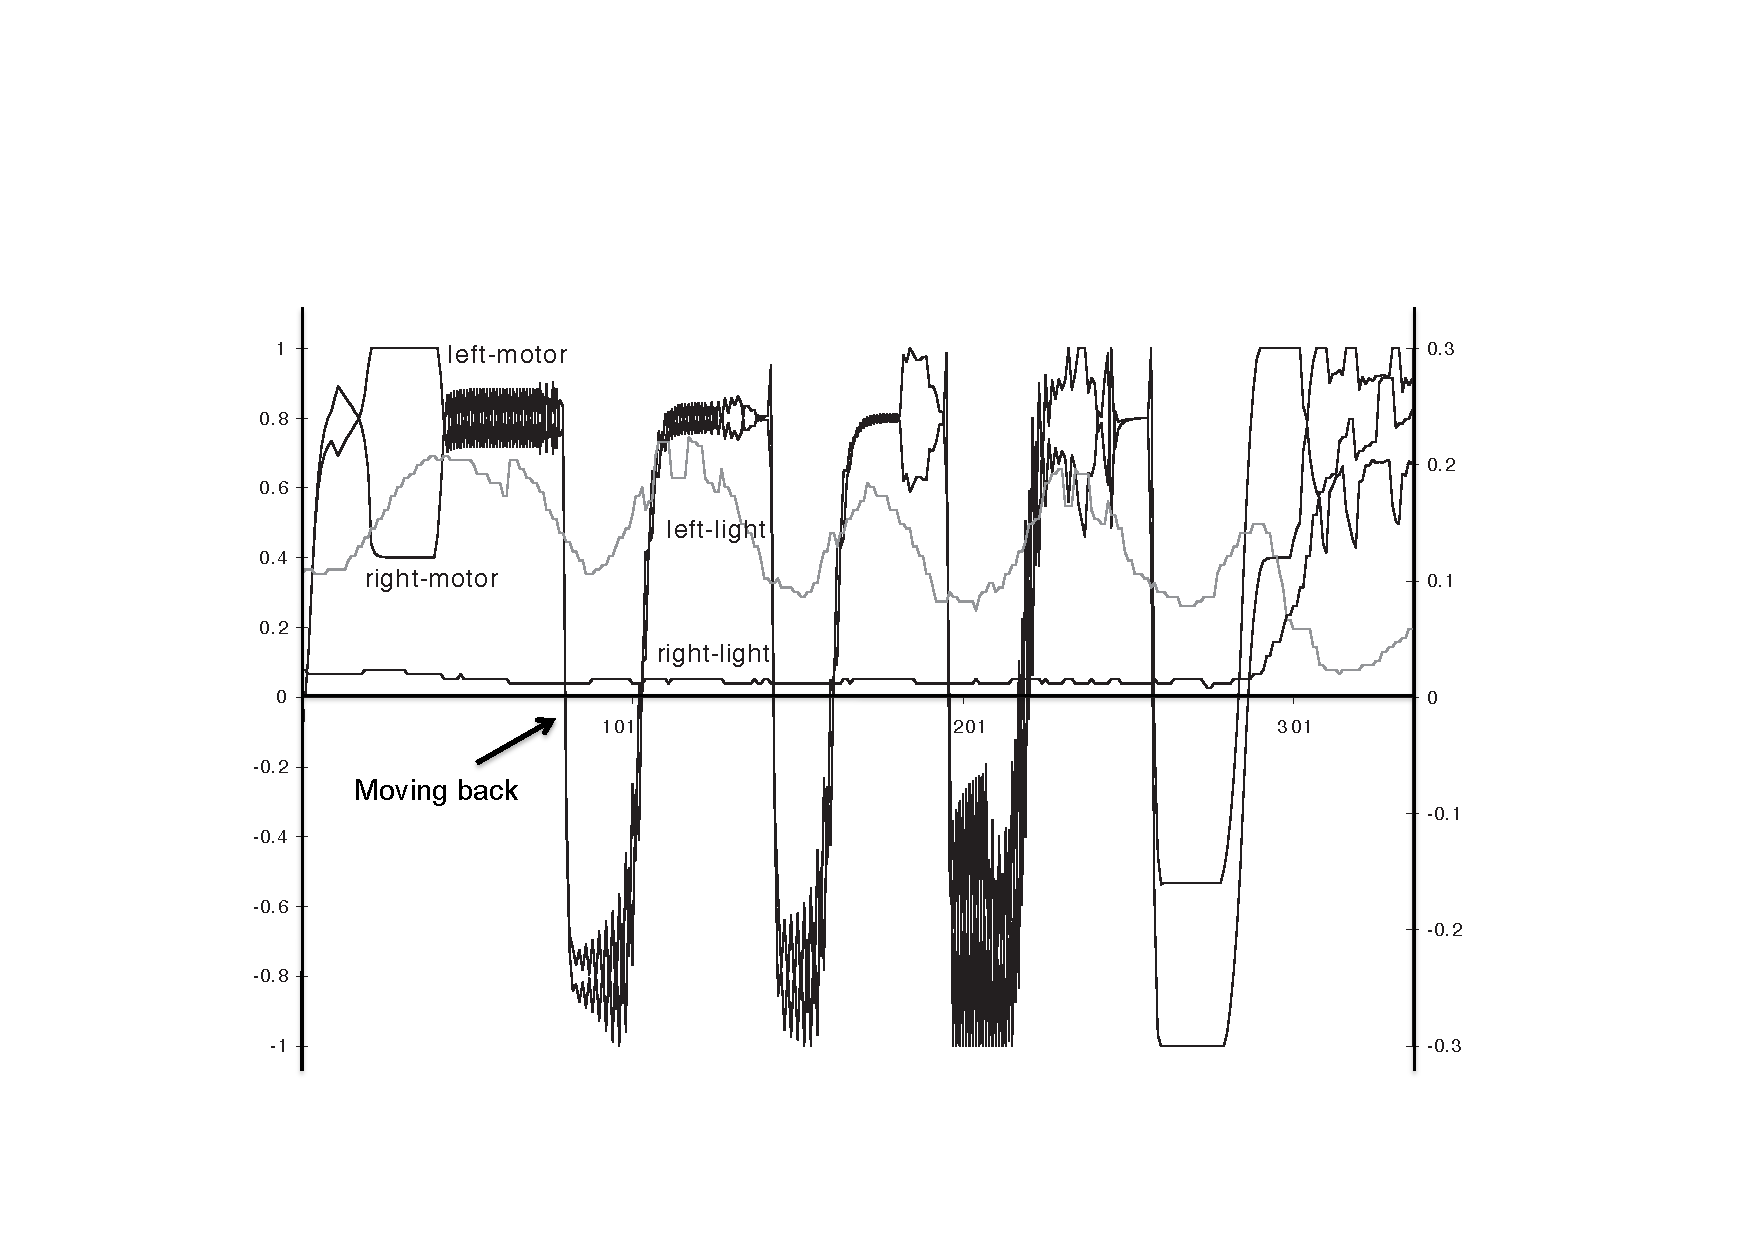
\includegraphics[width=.85\textwidth]{chap3/figs/phototaxis}}
\caption{\label{phototaxis} 
Internal states of a robot's sensory and actuator channels on 
the y-axis and time in periods of 1/40 second on the x-axis.
The robot pushes against a box holding a light source.}
\end{figure}

These channel recordings illustrate clearly that sensor or actuator
data is continuous in time and 
rapidly fluctuates in response to changes in the environment or the
behavior of the agents. Coupling sensory data to actuators
is effective for quick reaction
without the need for higher level processing. If 
an obstacle is rapidly approaching, it is important to get out 
of the way rather than trying to figure out what kind of 
obstacle it is. The observed behavior is very complex, even though
the underlying dynamical systems are relatively 
simple; the complexity is due to the complexity of the 
real world with which the robot is interacting. 

Similar behavior systems and networks have
been experimented with 
for more complex tasks and it is actually the way that 
the Mars rover discussed in the introductory chapter works.\footnote{At 
the risk of simplifying, we can say that the early 
work in cybernetics (such as that of Braitenberg
referenced above) has focused on this subsymbolic layer
and that `Artificial Intelligence' as a research field
emerging in the late fifties has focused on the 
symbolic layer. Some researchers involved in a bottom up 
approach to Artificial Intelligence strongly refocused
on the subsymbolic layer. One of the most
vocal advocates of this position is \cite{Brooks:1992}.
Obviously we need the two, 
but bridging the gap is a non-trivial problem, sometimes known 
as the grounding problem. See: \cite{Harnad:1994}. }
However, the gap between the continuous dynamics of sensori-motor
intelligence and cognition remains unbridged. 
It is possible for {\itshape us} to see 
structure in the data but this structure is not perceived
nor used for control by the robot itself. 
The robot does not segment nor categorize
reality. It does not `know' that it is moving left or right 
and therefore cannot communicate this information to another robot. 
All processing remains at the analog continuous
level. However because it remains at this subsymbolic level, it is doubtful
whether we can ever hope to bootstrap cognitive
intelligence simply by adding more of these dynamical 
systems.\footnote{
\cite{Marr:1982} remains a classical reference outlining
the features that can be extracted, the
principled algorithms for doing it, and possible 
neurophysiological models. These are the main research
topics that still dominate research in vision. See 
\cite{Ullman:1996} for a more recent overview.}
The difference between behavioral intelligence 
and cognitive intelligence resides in an additional 
layer of processing which is no longer continuous and analog 
but discrete and symbolic. How this second symbolic 
layer could be formed but at the same time remain 
grounded in the analog sensori-motor layer is one 
of the main research topics addressed in this book. 

\section{Segmentation} 

The first step that bridges the gap between sensory layers and \is{segmentation}
cognitive processing is segmentation. Segmentation means that 
a sensory data stream is divided into units 
either in space or in time. In the Talking Heads experiment, 
the environment is restricted to
static images only, so that segmentation
amounts to aggregating pixels into spatial patches.

A patch may have an irregular shape which makes it hard to apply 
some classifications without complex processing. Bounding boxes are much 
easier to compute and are already very useful. The bounding box of a segment 
is a rectangle around the contours of a segment (\figref{f:boundbox}).\is{bounding box} 
\begin{figure}[htbp]
  \centerline{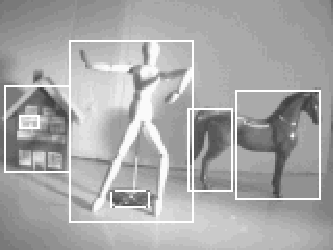
\includegraphics[width=.50\textwidth]{chap3/figs/sslang}}
\label{screenshot}
\caption{\footnotesize Example of a scene captured by the 
camera in \figref{f:plate7}, containing a puppet, a
wooden house, and a horse. Segmentation is based on aggregating grayscale
patches, i.e. areas in the image that are lighter or darker than the 
general background. Bounding boxes have been drawn around the segments. 
Note that there can be bounding boxes within bounding boxes if an object 
forms part of a larger object. 
\label{f:boundbox}}
\end{figure}

It is generally not necessary for segmentation to always yield parts of the images that correspond
to what we would call objects. This is an impossible demand. What counts as 
an object is to some extent task-dependent. 
Segmentation yields information that can be used for 
object identification but should not be equated with it. 
This is well illustrated in \figref{screenshot}. 
Segmentation has been done here by filtering out segments with 
lower or higher average grayscale values compared to the 
average in the scene. The segments that have been obtained
are not necessarily those that we humans identify, because we
use knowledge of the objects involved. This 
shows clearly that higher level constraints play a role 
even at the very first basic visual processing layers. 

\subsection{Feature extraction}

Many methods for segmentation have been reported \is{feature extraction}
in the computer vision literature and all of them are useful even though they 
give slightly different results. Most methods assume 
that additional low level processing is first performed 
on the image map to detect small-scale structures, such as: 
\begin{itemize}
\item Edges, which are possible boundaries between two 
surfaces. Edges can be aggregated in line segments. 
\item Junctions, which are regions where lines come 
together. 
\item Patches, which are regions where the colour or
the grayscale values are relatively constant. 
\item Textures, which are small-scale regular surface 
markings, for example blobs. 
\item Optical flow, which are vectors indicating the 
direction and velocity of moving brightness patterns. 
\item Distance from the observer, computed by
matching two image maps from binocular vision. 
\item Shadings, recovered from continuous variations in
brightness. 
\end{itemize}
The recovery of such features is in itself 
a non-trivial topic of research and a huge literature as well as 
many software libraries now exist.

The visual layer of the Talking Heads only extracts 
patches and edges which each leads to one way 
of segmenting the scene. 
Segmenting based on patches attempts to aggregate 
those parts of the image into patches (a process
called region growing) that have more or less the same 
colour. `More or less the same' is of course a relative
notion and larger or smaller segments will be found
depending on the thresholds that are used for 
deciding whether a colour is similar or not. Segments
that are too small are not considered further. 
Region growing starts by comparing for each pixel how similar it is to 
neighboring pixels. Similar pixels
are grouped as a patch. In the next step, each patch
is examined to see whether it can be merged with
a neighboring patch, and so on recursively until 
patches cannot be combined further. Small patches or individual pixels that 
stand on their own are included as part of a larger
patch so that we get sufficiently broad patches. 

Segmentation based on edges starts by first detecting the 
edges themselves, which are colour discontinuities suggesting a boundary
between two surfaces. The edges are then aggregated into lines, and these lines are 
connected to find the contours 
of an object. This method works well for the simple 
objects used in the Talking 
Heads experiment. Things are
no longer so simple when contours are less
clear, for example because they fuse with the background. 
Further complications arise when one object partly obstructs
another object or when a set of lines can ambiguously 
be organised in different configurations (as in visual illusions
like the Necker cube). This illustrates that one 
segmentation method must be balanced with others to offset unclear 
areas or local ambiguities. 
\begin{figure}[htbp]
  \centerline{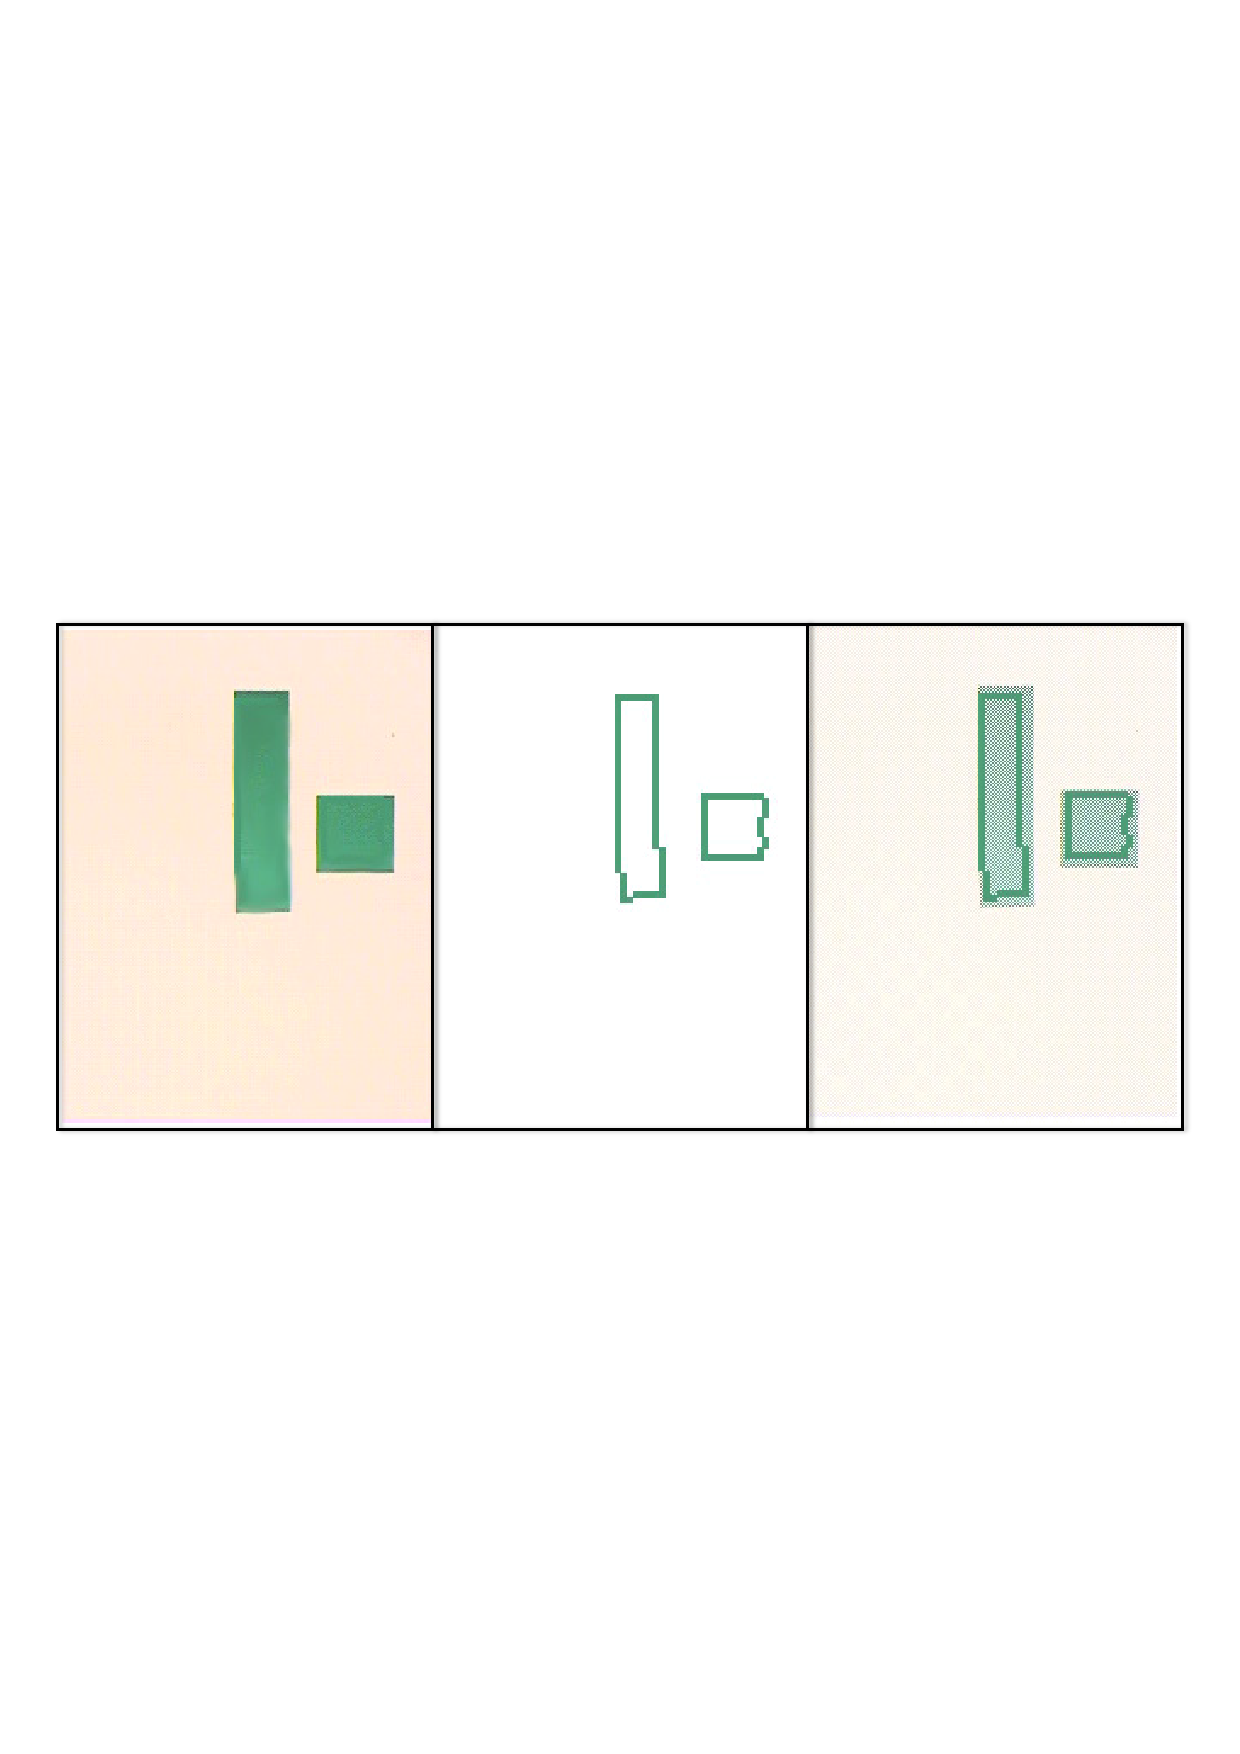
\includegraphics[width=.75\textwidth]{chap3/figs/image1}}
\caption{ Left view shows an image as captured by a Talking
Heads camera. Middle view shows the result of 
segmentation based on edge detection. Right view
shows the integration of segmentation by color
and by edge detection.}
\label{f:plate11}
\end{figure}

The results of applying these two segmentation methods
can be seen in \figref{f:plate11}. 
The top picture shows the image map itself as it is captured by 
a Talking Head camera. The middle image shows the result of 
segmenting based on edge detection. The contours of two 
objects have been found. Note that these contours are not 
straight lines as one might expect. They are obtained by 
connecting together line segments which are themselves 
based on connected edges. The bottom image shows the combination of 
edge detection and segmentation based on patches. Because the green 
objects stand out clearly against the white background
they are easily recognised by the combination of 
these segmentation methods. Given the simplicity of the Talking Heads
environment (geometric shapes on a white board),
segmentation based on colour and on edge detection
generally yields a segmentation that corresponds 
to the individual objects humans perceive in a scene. 

\subsection{Divergent perception}
\is{divergent perception}

There is no guarantee that two Talking Heads
looking towards the same area of the white board
perceive exactly the same image. In fact, the contrary 
is true. Because the robots are physically grounded 
and situated in a particular context, standing roughly one 
meter apart from each other \figref{f:plate1}, they cannot 
see the same scene from exactly the same vantage point, and 
so images diverge. On the edges of the field of view, 
the differences might become so significant that 
different objects are seen and consequently different
categories used. 

Compare for example the recorded images for a speaker (top)
and a hearer (bottom) as shown in \figref{f:plate12} (to the 
left). The same Figure shows the segmentation performed by 
both agents in a separate window (to the right). The images
are clearly different because they have been taken from 
slightly different camera positions and the hearer only approximately
perceives in which direction the speaker is pointing. 
Agent {\bfshape a1} (top of \ref{f:plate12}) has recovered the two circles, but
not the rectangle which was deemed to small to be relevant. 
Agent {\bfshape a2} (bottom of \ref{f:plate12}) has recovered the rectangle 
in the left top corner but only one circle. The yellow circle
was not recognised by {\bfshape a2} due to slightly different 
reflections perceived from {\bfshape a2}'s angle of view, so that the yellow 
surface was no longer distinguishable from the white background. 

Usually the situation is not so divergent, and even 
if there is divergent perception, the categorisation
used by the speaker may still be compatible with the 
same topic for the hearer. Nevertheless, we must take into account that divergent perception 
of the scene might considerably confuse language communication and the feedback the speaker gives
to the hearer. This is one example where it is useful to do grounded experiments because it shows 
clearly a major issue (namely perceptual and hence categorical divergence) which is usually swept 
under the carpet. 

\begin{figure}[htbp]
  \centerline{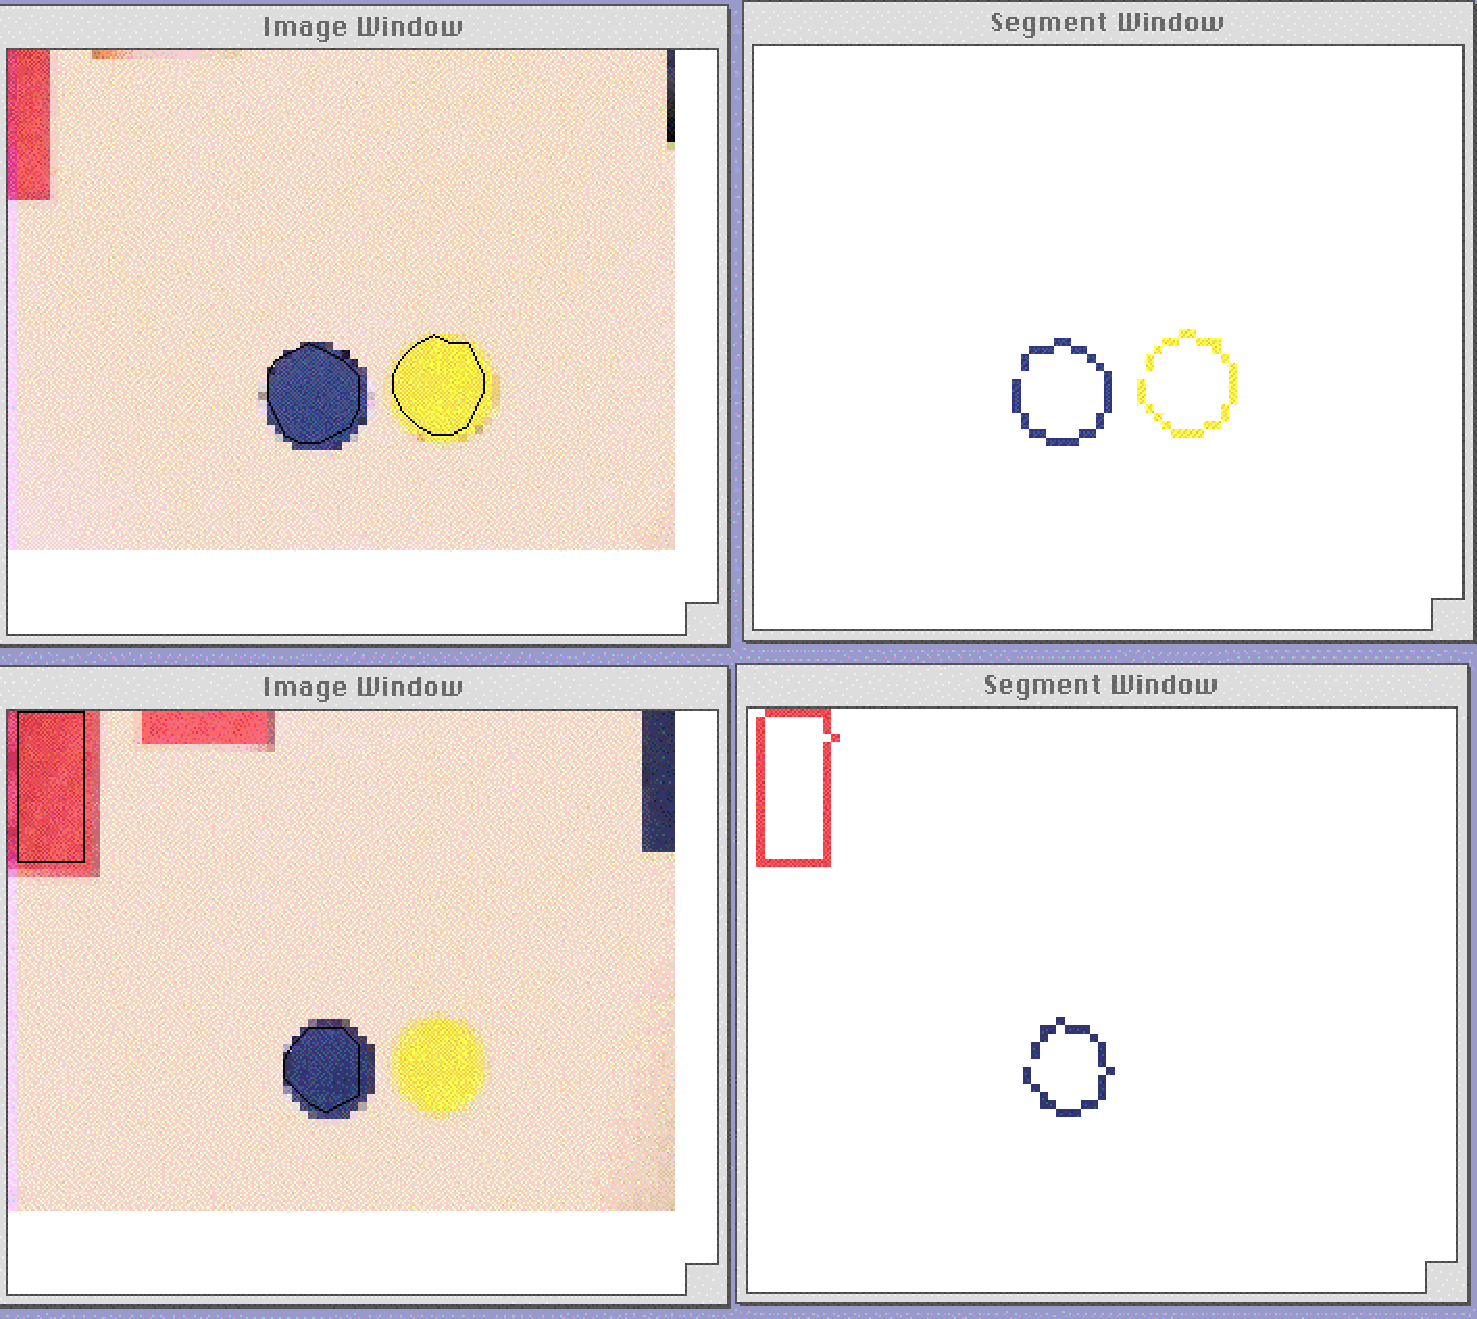
\includegraphics[width=.55\textwidth]{chap3/figs/diff-percept}}
\caption{ Top (left), image captured by the hearer. 
Bottom (left), image captured by the speaker. Because
both have a different view on the scene, the 
images diverge and consequently 
the segmentation (bottom and top right) diverges as well, in particular the yellow 
circle is not perceived by the speaker. In contrast the speaker perceives a rectangle
(bottom left corner) and has chosen this as the topic. The rectangle is not perceived by the 
hearer, so the game has no chance to be successful.}
\label{f:plate12}
\end{figure}

\subsection{The Sieve Architecture}

\is{sieve architecture}Segmentation exemplifies a dual kind of processing that 
we will encounter again and again as we focus on the 
different layers of the cognitive 
architecture (\figref{f:sieve}). 
Various possible solutions are generated, 
expanded and combined in parallel. The possible solutions enter
into competition until globally coherent
solutions emerge, which are ranked and handed to the 
next layer of processing. Often 
a solution does not emerge or multiple solutions are
equally valid in which case constraints from 
expectations or from the further processing of partial
solutions must flow down to influence `earlier' processing, 
which can be implemented as a `re-entry' of some solutions
back into the previous layer. For example, hearing a word may 
stimulate the expectation that a certain category is
relevant, which in turn may stimulate the computation
of certain features and influence how the image is 
segmented. A speaker may have to choose between alternative
segmentations and categorisations depending on whether 
the conceptualisation can be succinctly and accurately 
lexicalised and possible lexicalisations will only be 
acceptable when they can be integrated in a complete sentence. 
\begin{figure}[htbp]
  \centerline{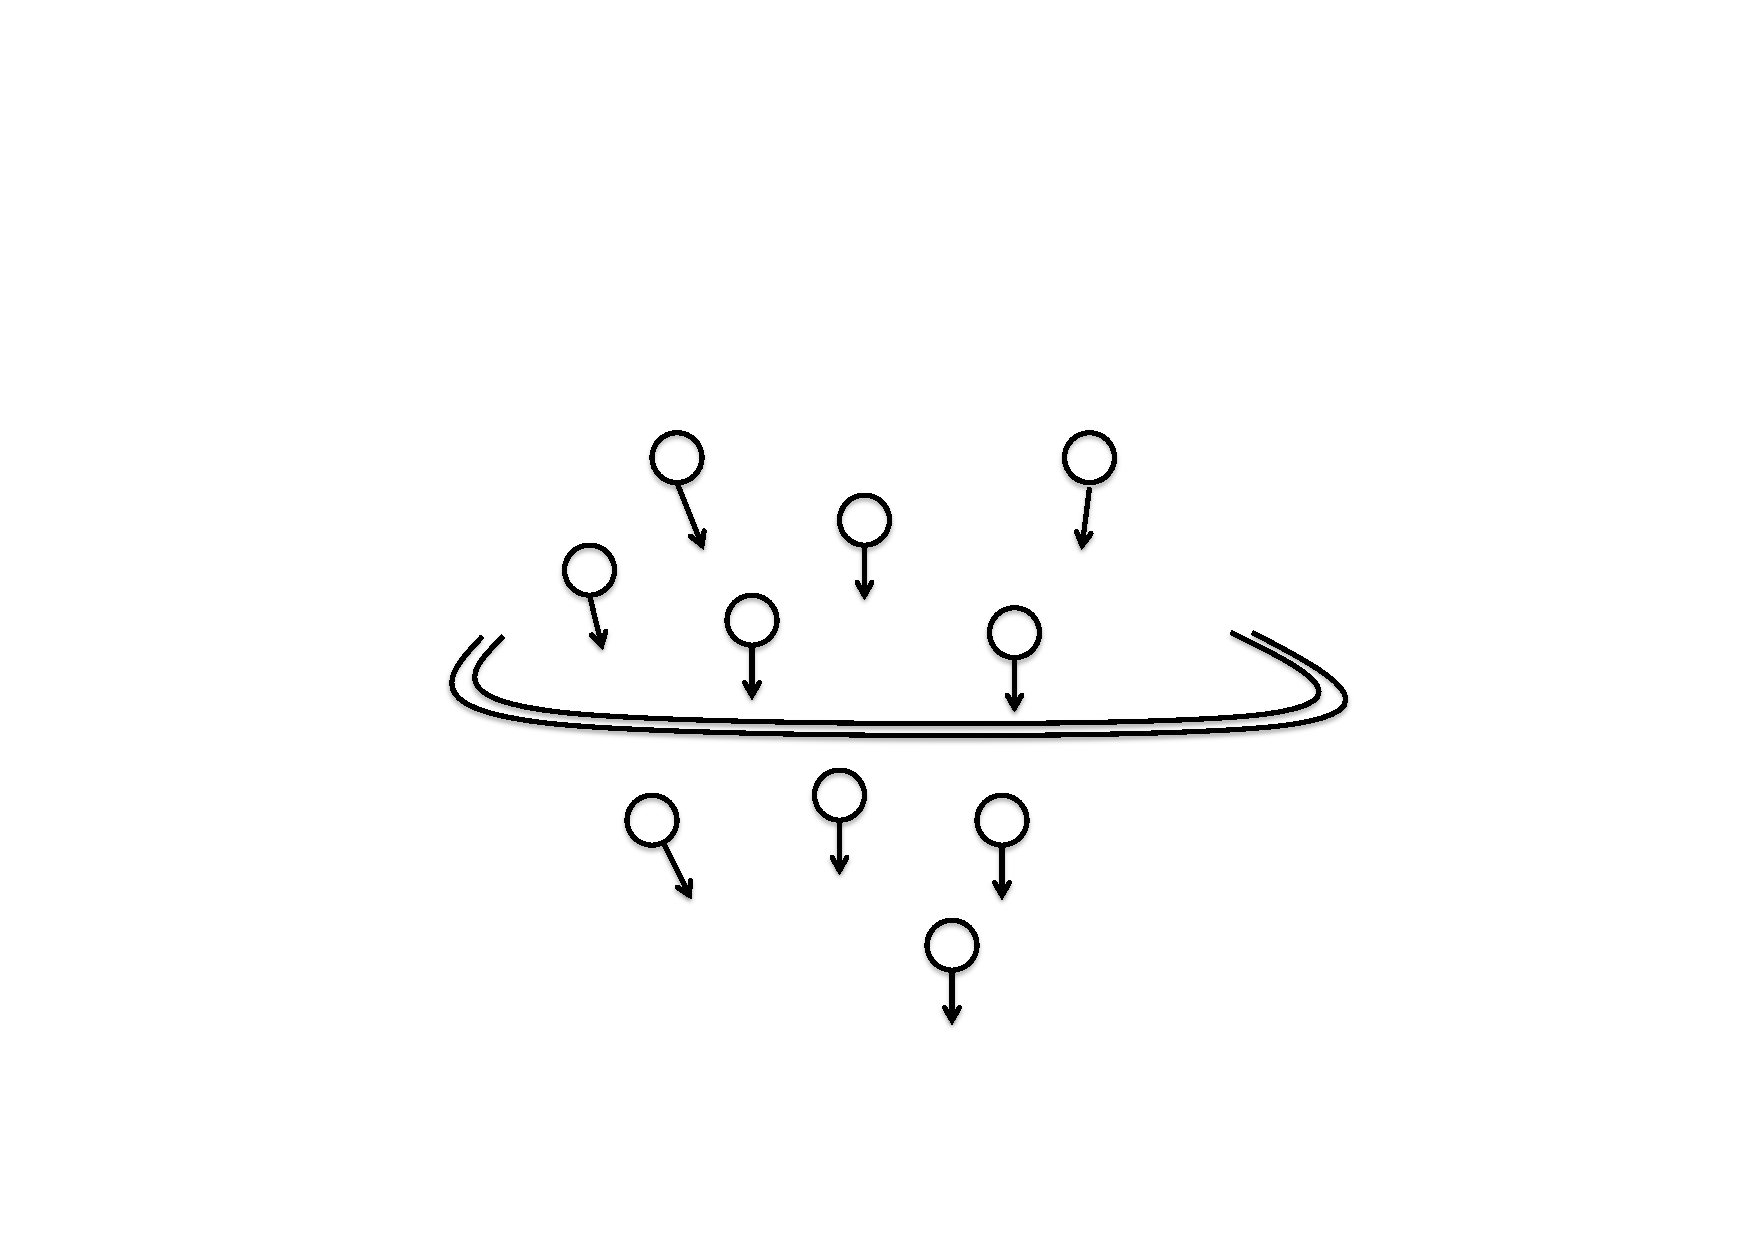
\includegraphics[width=.55\textwidth]{chap3/figs/sieve}}
\caption{\footnotesize The different layers of cognitive processing act 
like a sieve. Inputs flow into the layer, where they are processed
to generate hypotheses of which the best ones are transmitted
to the next layer. Every layer can operate in both directions, 
so that constraints can flow from top to bottom and from bottom
to top. \label{f:sieve}}
\end{figure}

The two way flow of constraints (from perception to 
high level cognitive processing and from high level 
cognitive processing to perception) suggests 
that the brain is best thought of as a massively parallel, 
densely connected processing system, in which multiple 
partial solution structures float up or down, gathering strength 
or weakening with new information entering the system. 
This contrasts with the view that 
information is processed in a serial step-by-step fashion
through tightly compartmentalised modules.\footnote{
See \cite{Fodor:1983} This book discusses a modular, sequential 
information processing architecture for cognition. A 
non-modular, parallel view 
is sketched in: \cite{Minsky:1985}. 
A more realistic neurophysiological model similar to the 
one underlying the `sieve architecture' we have used is
discussed by \cite{Edelman:1987}.} It is true
that we have the illusion that there 
is some {\itshape homunculus}, a little man, which sees a single coherent 
picture of reality and finds quickly the right way to 
verbalise or interpret this picture, but closer examination 
of the actual informational requirements of each subprocess
shows that this can never work. Constraints must flow in all 
directions, because the sensory data has not enough information to allow 
a unique segmentation, and categorisation and language is 
too full of ambiguities to allow a straightforward linear
interpretation. 

\section{Sensory Channels}

\is{sensory channels}Once segments have been found, further characteristics must
be extracted. The values of these various characteristics
will be communicated on sensory channels to later categorisation
processes. A characteristic property of a segment, such as 
average gray-scale, is still in the
analog continuous domain and should not be confused with
a category (like dark or light) which is in the
discrete symbolic domain. An open-ended set of possible sensory 
channels can be imagined, ranging from very general 
channels sensitive to often recurring properties relevant
in common tasks and thus shared by most people, to very 
specific channels which only experts in specific
domains possess. 

\subsection{Example channels}

The segment characteristics which will be 
used later in various experiments are defined below. 
Their values are all derived by straightforward computations from 
the raw image maps captured by the cameras. 
\begin{itemize} 
\item AREA: The surface area of a segment
is calculated by simply counting the number of pixels that are part 
of the segment. 
\item HPOS, VPOS: The x and y values of the 
central-position of a segment. The central position 
is calculated by taking the mid-point of the sides 
of the bounding box. 
\item HEIGHT: The height of the bounding box. 
\item WIDTH: The width of the bounding box. 
\item BB-AREA: The area of the bounding box,
calculated by multiplying height by width. 
\item GRAY: The average gray-scale value of the pixels
in a segment. 
\item R, G, B: The average R (redness), G
(greenness), and B (blueness) values in a
segment. To obtain more human-like colour channels, they are
transformed in terms of YB (yellow-blue), RG (red-green), 
BW (black-white), SAT (saturation) and BRIGHTNESS channels. 
\item EDGE-COUNT: The number of edges in
a segment, for example 3 in the case of 
a triangle. 
\item ANGLE-COUNT: The number of angles, determined on the 
basis of the junctions. 
\item RATIO: The ratio between the area of the segment 
and the area of its bounding box, which gives an idea how close 
a figure is to a rectangular shape. 
\end{itemize}

Each of these segment characteristics or combinations of
characteristics enables certain types of
categorisations. For example, the GRAY channel makes 
it possible to distinguish between 
light and dark, HEIGHT between short and tall, HPOS between 
left and right, VPOS between top and bottom, 
AREA between big and small, etc. In the next chapter, we will study 
how such categorisations may 
form on the basis of their respective channels. 

\subsection{Conceptual spaces}

\is{conceptual spaces}The sensory channels used in the experiments have
deliberately been kept to a minimum so that we can follow 
in detail the ontological and lexical dynamics, which is a 
non-trivial matter as I will demonstrate in chapters 6 and 7.
Obviously to get a richer lexicon, more channels need to be made 
available to the agents. These channels can often be 
grouped to form a `conceptual space'.\footnote{See \cite{Gardenfors:1999}
More cognitive oriented spaces, further removed 
from perception, are discussed in \cite{Fauconnier:1994}.} One of the 
best known examples is the colour space formed by the
yellow-blue, red-green, black-white, saturation, and brightness channels. 

Here are some other examples: 

1. A set of sensory channels that are sensitive 
to characteristics of moving segments can easily be 
imagined. They include the speed
of movement, the direction of movement (along the 
horizontal position (HPOS) and vertical position (VPOS) 
dimensions), or the change in area (getting bigger if the object 
approaches or smaller if it moves away). This is the foundation
for categories about spatial change: moving left versus moving right,
approaching versus retracting, speeding up versus slowing down.\footnote{Experiments
using segmentation based on movement
using the dedicated hardware shown in \ref{f:plate6} were carried out by Tony Belpaeme. 
More details can be found in: \cite{Belpaeme:1998} These channels have been used in
language experiments where the agents were 
perceiving and communicating about moving 
images: \cite{Steels:1998}  
The segmentation used in this book 
based on output from the Sony EVI-D31 camera was 
implemented by Danny Van Tieghem. Angus McIntyre integrated
the interfaces to this camera within the BABEL environment. 
}

2. Various spatial relations between segments can be computed: 
inclusion and overlap between segments, distance between 
midpoints, hierarchical structure, etc. 
This leads to another batch of categories which are
the basis for spatial distinctions like inside versus outside. 

3. More properties of the shape of segments can be computed.
I have already introdced the RATIO channel, which is the area of the 
segment divided by the area of the bounding box, giving an 
indication how rectangular a segment is. This can be generalised
by using an ellips around a shape so that we can calculate
convexity. We can then also calculate elongation (by calculating
the principal axes of the ellipse). 

It is not at all necessary that the channels operate 
on visual input, they can also use actuator sensors or internal states
like the level of the battery. It is moreover possible to 
consider channels for dynamic states, for 
example by transforming the sensor and actuator
data into state-space representations and 
analysing them in terms of attractors.\footnote{
Several examples of this type of approach are 
found in \cite{Port:1995}}

The ontological and lexical apparatus of the Talking Heads is 
generic with respect to the nature of the sensory channels
that are used, they could just as easily be about other sensory 
domains like sound, tactile sensation or internal states
of the robots.

\subsection{Perceptual Constancy}

\is{perceptual constancy}Real world sensory data is remarkably volatile due to the 
high variation and constant change of 
our physical environment, nevertheless human beings have 
the illusion of constancy. 
For example, the colour of an object is determined 
by the wavelength of the light reflected by its surface. 
For a long time, it 
was thought that colour was an intrinsic property of a 
surface, and that we therefore experience the colour of 
an object as constant, but psycho-experimental evidence has shown 
that this is not true. When we look at a surface in 
isolation which reflects light between 
430 and 470 nanometers, we experience 
the colour blue. As a result, one might assume
that blue can be equated
with the experience of light in this particular wavelength 
region. However, if the same surface is perceived
in a broader context and the light conditions 
are changed (so that objectively they now 
reflect light in a different spectral region), they still 
appear as blue! What should objectively 
appear green according to the measured wavelength 
values is still experienced
as blue. This explains why we see colours
as relatively constant even if the light conditions
are changing (for example from broad daylight to 
evening light) which is obviously extremely useful 
for dealing with rich environments. But it 
implies that colour is {\itshape not}
an intrinsic property that can be measured objectively 
with a light meter. It is actively mapped onto reality 
as a result of complex processing which takes the 
context into account.\footnote{
See the discussion about colour 
in: \cite{Varela:1991}}

The same sort of context-sensitivity\is{context-sensitivity} 
is important for the other sensory dimensions 
that the Talking Heads use, as well as for segmentation. An 
object will appear large or small depending on the 
other objects in the scene. It will appear light 
or dark depending on the average brightness. 
A scene may be segmented in one way or another 
depending on the objects it contains. 
Visual illusions arise when more than one context
is consistent with an image and interpretations sometimes
switch back and forth between different possibilities. 

\subsection{Transformations}

Cognitive agents can stabilise the sensory data to
achieve more perceptual constancy by transforming them so 
that the data become less context-sensitive. 
This implies that additional processing first recovers
more information about the context. 
One of the best known examples of this concerns
colour constancy. As mentioned earlier, wavelength 
reflection is strongly influenced by the background 
light in the environment. However, when the average surface 
reflectance is known, it is possible to transform 
the colour data to recover the colour that is 
experienced by humans as constant for a surface.\footnote{
See the discussion in: \cite{Zeki:1993}, particularly chapter 
23.}
 
\subsection{Scaling}

\is{scaling}The second way in which the erratic nature of 
real world signals can be diminished is by
scaling. Scaling means that 
the values actually recorded by sensors or
feature extractors are calibrated with respect 
to a frame of reference. 

A first frame of reference is based on
the absolute minima and maxima of the values 
on a sensory channel. This can be used to do 
{\itshape sensor-oriented scaling}. For example, 
the image map captured by the camera
contains 320 x 240 pixels, which means 
that the horizontal position (HPOS) has a value between
0 and 320 and the vertical position (VPOS) has a value 
between 0 and 240. Both values can be scaled to fall between 
0.0 and 1.0 so that they become uniform with respect to 
other sensory channels. Given a value $x$ and a 
$min$ and $max$ value, then the scaled value is 
$x' = {(x - min)}/{(max - min)}$. 
Thus the sensed value of HPOS=200 becomes
HPOS=0.62 after scaling . 

In the experiments discussed later, 
sensor-scaling is always performed so that all sensory data
is between 0.0 and 1.0, allowing values on different channels 
to be compared with 
each other. In addition, context-oriented scaling is performed.
{\itshape Context-oriented scaling} uses the minima and maxima of the 
values that effectively appear in the context.
For example, if the values for the HEIGHT of segments 
observed in the scene is between 500 and 700, 
then these can be the minimum and maximum of the 
HEIGHT scale, so that 500 maps onto 0.0 and 700 to 1.0. 
Context-oriented scaling acts like a lens
magnifying the perceived values so that distinctions
stand out more clearly. This scaling could 
be made more sophisticated by introducing an additional scaling factor so that 
differences are amplified but not necessarily blown up to their extremes. 

Context-oriented scaling has two advantages. The 
context is now strongly taken into
account, in a way similar to human perception: A segment
looks dark when surrounded by light segments but
light when surrounded by darker ones. The second advantage is 
that differences within the relevant subrange that 
actually occur in the scene are amplified, so that 
they stand out even if the range of possible values is
much wider. Often both relative (context-oriented) 
and absolute (sensor-oriented) scaling 
are pertinent. Thus `left' can be
the left-most of all the objects in the scene (context-oriented
scaling) or `left' in absolute terms (sensor-oriented scaling). 
Some channels, such as the colour channels, should never be scaled
for context, because the categorisation works best on the basis of 
the sensor-scaled values. 

Context-oriented scaling is not necessarily based on the 
frame of reference imposed by the image map which is 
recorded by perceiving the scene from the viewpoint of 
the camera. Many contexts and hence other frames of reference
are possible and are exploited in natural language 
conversations. Often a particular context is communicated through 
language. Scaling is then performed within the
frame of reference suggested by that context, 
for example, if I will tell someone "the chair is to
your left", whereas it may perhaps be to the right of the
hearer from my point of view. 

A final form of scaling uses the typical values of the object being 
perceived. I will call this {\itshape object-oriented scaling}. 
For example, a small elephant is always
very large next to a large mouse. We clearly
have expectations about the typical size of an elephant at
a certain distance and use it to scale
perceptual data prior to size 
categorisation. Context-oriented and object-oriented scaling
are examples how constraints must flow 
from non-visual cognitive processes to visual processing. 
These non-modular interactions are a strong
indication that cognitive subsystems must be highly 
interconnected. 

\subsection{Saliency}

\is{saliency}The perceptual layer generates in parallel a wealth of 
sensory characteristics about each of the segments in 
an image and their relationships. But not all sensory 
characteristics are equally distinctive. For example, two 
segments in a scene may have almost the same area but 
one might be very thin and thus tall, and the other very wide
and thus short. In our own human perception, those channels
that reflect significant differences stand out and are preferred
in referring to an object. Therefore, it is unlikely that area would be 
used in \figref{rect1b} to distinguish object 1 from 
the others. 
\begin{figure}[htbp]
  \centerline{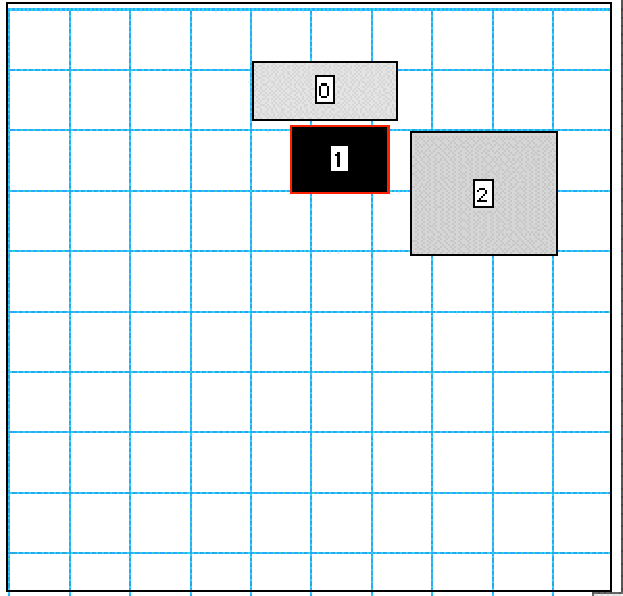
\includegraphics[width=.45\textwidth]{chap3/figs/recscene}}
\caption{\footnotesize \label{rect1b} A scene with three objects. The
sensory values on the grayscale channel are the most salient 
and will therefore be chosen preferentially for categorisation
and verbalisation.}
\end{figure}

The saliency of a channel 
is the smallest distance (after sensor-scaling) between the perceived
values of the topic and one of the corresponding perceived values of the 
other segments in the context. 
Thus the different perceived values (after sensor-scaling)
for the segments in \figref{rect1b} are shown in 
\tabref{tab:rect1b}. The last line shows the saliency, assuming that 
the topic is segment 1.  Clearly the GRAY-channel is the most salient
one in this case, followed by the WIDTH-channel. Other 
sensory channels such as HPOS, VPOS or HEIGHT (which have almost the same 
values for object 0 and 1) are not salient at all. 

\begin{table}
\begin{center}
\begin{tabular}{  l   l   l   l   l   l   l  }
\lsptoprule
{\itshape obj} & HPOS & VPOS & HEIGHT & WIDTH & GRAY & AREA \\ \midrule
0 & 0.66 & 0.95 & 0.01 & 0.71 & 0.19 & 0.27\\ 
1 & 0.69 & 0.83 & 0.07 & 0.33 & 0.97 & 0.21\\ 
2 & 0.99 & 0.87 & 0.54 & 0.72 & 0.22 & 0.57\\ 
sal & 0.03 & 0.05 & 0.07 & 0.39 & 0.75 & 0.06 \\ 
\lspbottomrule
\end{tabular}
\caption{Perceived values for each segment in \figref{rect1b}.
\label{tab:rect1b}}
\end{center}
\end{table}

Determining saliency has to be done before context scaling, because
context-scaling stretches the values to their extremes and so 
saliency information is lost. 
\tabref{tab:rect1b-area} below shows for the scene shown in
\figref{rect1b} the AREA channel with its
raw data, the value after 
sensor-scaling (with minimum 1,000 and maximum 
10,000), and the value after context-scaling. 
\begin{table}
\begin{center}
\begin{tabular}{  l   c   c   c  } \lsptoprule
{\itshape Object} & {\itshape Raw data} & {\itshape Sensor-scaled} &  {\itshape Context-scaled} \\ \midrule
0 & 24530 & 0.27 & 0.18 \\ 
1 & 18924 & 0.21 & 0.0\\ 
2 & 50960 & 0.57 & 1.00 \\ 
\lspbottomrule
\end{tabular}
\caption{Data for the area channel for the scene in \figref{rect1b}.
\label{tab:rect1b-area}}
\end{center}
\end{table}
\begin{figure}
\begin{center}
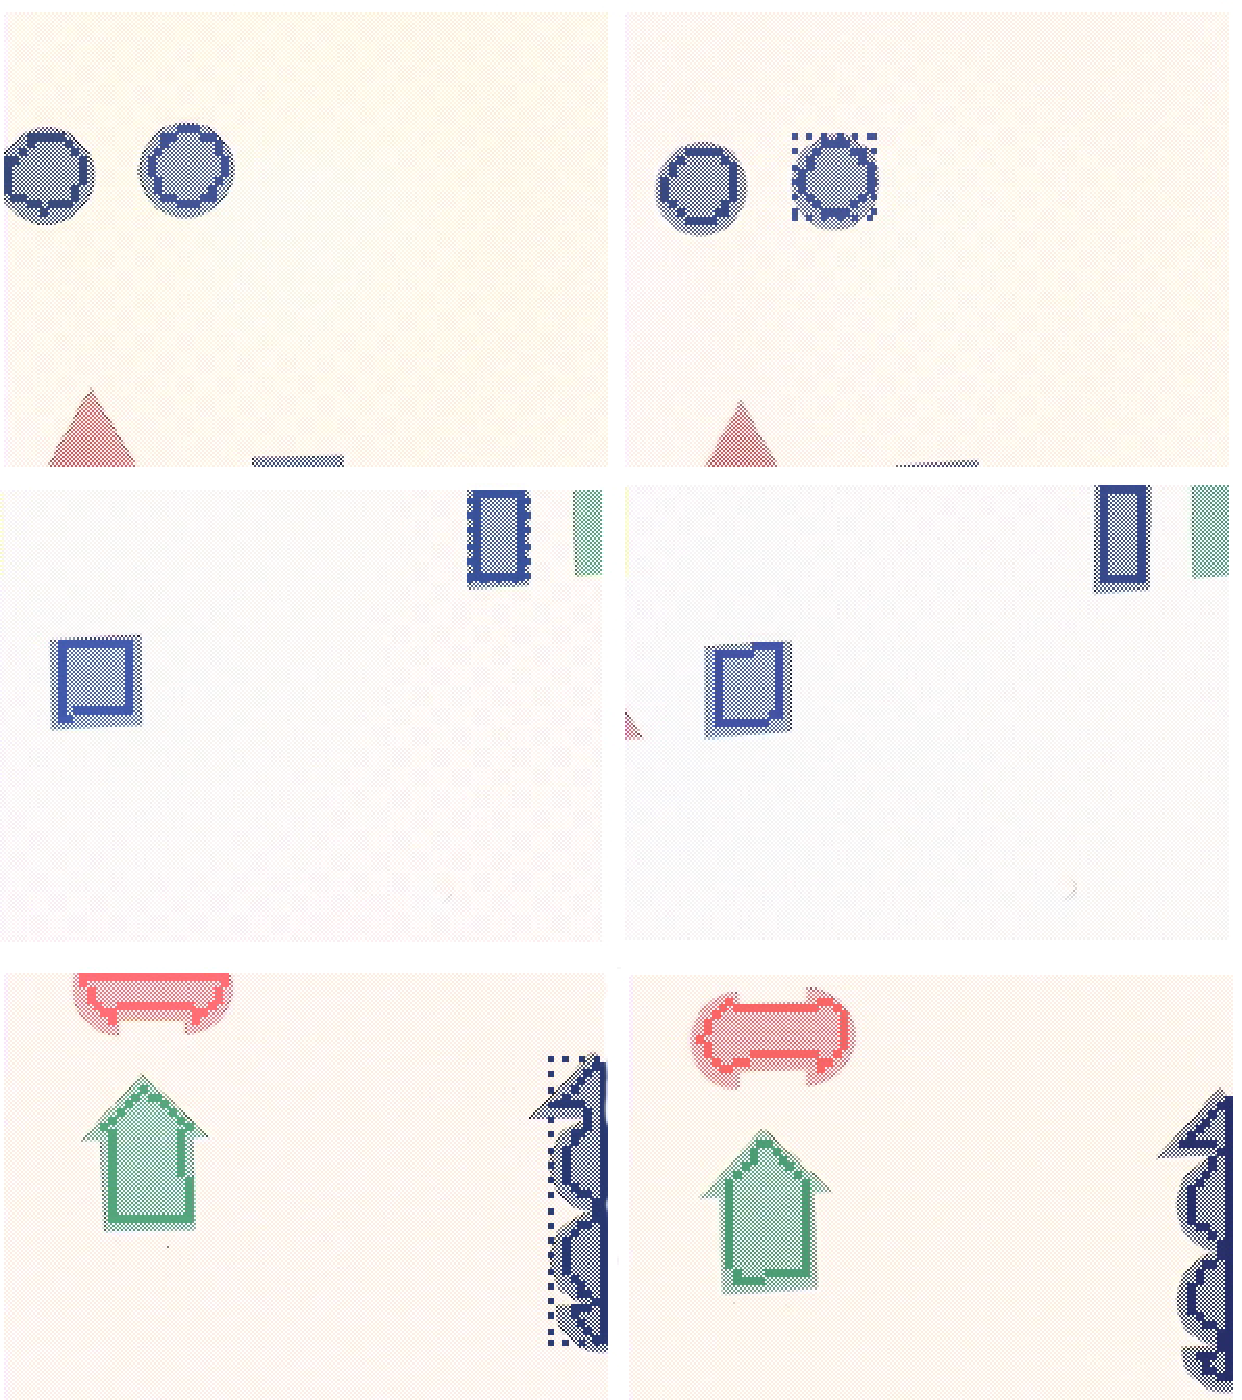
\includegraphics[width=0.8\columnwidth]{chap7/figs/plate-10}
\end{center}
\caption{Three examples of segmented images. The 
topic is indicated by a dashed bounding box in the 
image of the speaker. Segments which are too small 
are ignored. The topics have all been conceptualised
as being `to the right' and so the same word 
"gofubo" has been used to refer to them. }
\label{f:plate-10}
\end{figure}

Another example based on the segmented image is shown in Figure 
\ref{f:plate-10} (top images). Two circular segments
have been identified, the others are ignored because they are 
too small. The different sensory values (after sensor-scaling)
for the segments in the speaker's image are shown in \tabref{tab:t-plate10}. 

\begin{table}
\begin{center}
\begin{tabular}{  l   l   l   c  } \lsptoprule
{\itshape channel}& {\itshape obj-0} & {\itshape obj-1} & {\itshape saliency}\\ \midrule
HPOS & 0.27 & 0.16 & 0.11\\ 
VPOS & 0.20 & 0.20 & 0.0\\ 
HEIGHT & 0.15 & 0.15 & 0.0\\ 
WIDTH & 0.10 & 0.11 & 0.01\\ 
AREA & 0.10 & 0.10 & 0.0\\ 
R & 0.23 & 0.25 & 0.02\\ 
G & 0.32 & 0.34 & 0.02\\ 
B & 0.63 & 0.65 & 0.02\\ 
\lspbottomrule
\end{tabular}
\caption{Perceived values for each segment in \figref{f:plate-10}
\label{tab:t-plate10}}
\end{center}
\end{table}

The table shows clearly that HPOS is the most salient channel. 
The horizontal position also strikes us immediately 
as being the most salient when looking at plate [game2]. 
For many of the other channels, the differences are
almost insignificant. The use of saliency facilitates 
enormously communication and the acquisition of new categories. 
The case shown in plate 10 (top images) is an excellent opportunity 
for the agents to learn about left versus right. If more 
channels are salient, it is no longer so easy for the 
hearer to guess what meaning might have been used by the 
speaker and so incoherence would slip into the group's lexical
system. 

\begin{figure}[htbp]
  \centerline{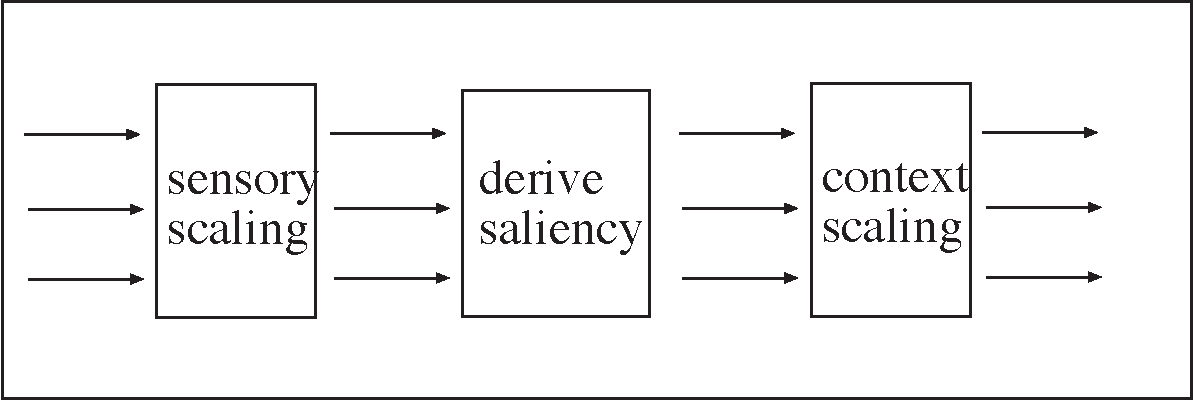
\includegraphics[width=.65\textwidth]{chap3/figs/scaling}}
\caption{\label{scaling} Processing converts data on 
a sensory channel into more usable data for later categorisation processes.}
\end{figure}

The various steps that the agents go through
in preparing data on sensory channels are summarised in \figref{scaling}.
It is presented here as flowing in one direction, but in fact 
constraints coming from higher level cognitive processing may 
influence these steps. For example, if we say "the largest square 
left of the triangle", we expect the hearer to scale the squares
with respect to all the objects left of the triangle, not with 
respect to all the objects in the scene. The backward flow of 
constraints will be studied after I have covered the different 
layers separately. 

\section{Methodology}

I hope the reader now has a much better idea of the enormous challenge
that the Talking Heads face when trying to play a language 
game about a real world scene, particularly
because they try to develop a lexicon and ontology 
as well. The images contain a multitude of ways 
to make distinctions and they differ slightly for both agents. 
It is enough fo a cloud to pass by causing the light conditions
to change slightly, and different values are immediately seen 
on the colour channels possibly leading to different segmentations.
So how can the agents ever get a repertoire of abstract categories and 
associated words when the real world shows such a perplexing 
variation? Very different scenes (for example the ones contained
in plate 10) can intuitively be distinguished with the same 
categories (namely [LEFT] versus [RIGHT]). But how can such 
inductive leaps be made? Scaling and sensor transformation 
introduce some perceptual constancy, and saliency helps to 
restrict the attention to those
channels that are potentially effective in communication, but there 
is clearly an enormous gap between sensory data and language. 

In this book, I will 
not only report on the outcome of an experiment and 
what we learned about the nature of cognitive architectures, but 
I will also try
to illustrate how we tackle such tremendously complicated problems. 
I will take a moment to explain this methodology because it runs like 
a red thread through the remaining chapters of this book and 
differs from the way other subdisciplines of cognitive science 
go about their investigations. 

\subsection{Putting up scaffolds}

\is{scaffolds}The standard means of attacking a difficult problem is to 
break it up in subproblems. In this case, the most obvious
subdivision is along the different sides
of the semiotic square I introduced in the 
previous chapter (\figref{square}). This 
leads to three natural subproblems: perception, conceptualisation, 
and verbalisation. When breaking up a problem, we can initially assume that the 
other subproblems will be solved somehow and that they give perfect
output to the others
or provide the right feedback. We can then try to invent a mechanism that
can do the job for the subtask we are investigating in these ideal circumstances, 
and test its strength and limitations. This is like putting up
scaffolds to see whether partial solutions work, before putting 
it all together. 
\begin{figure}[htbp]
  \centerline{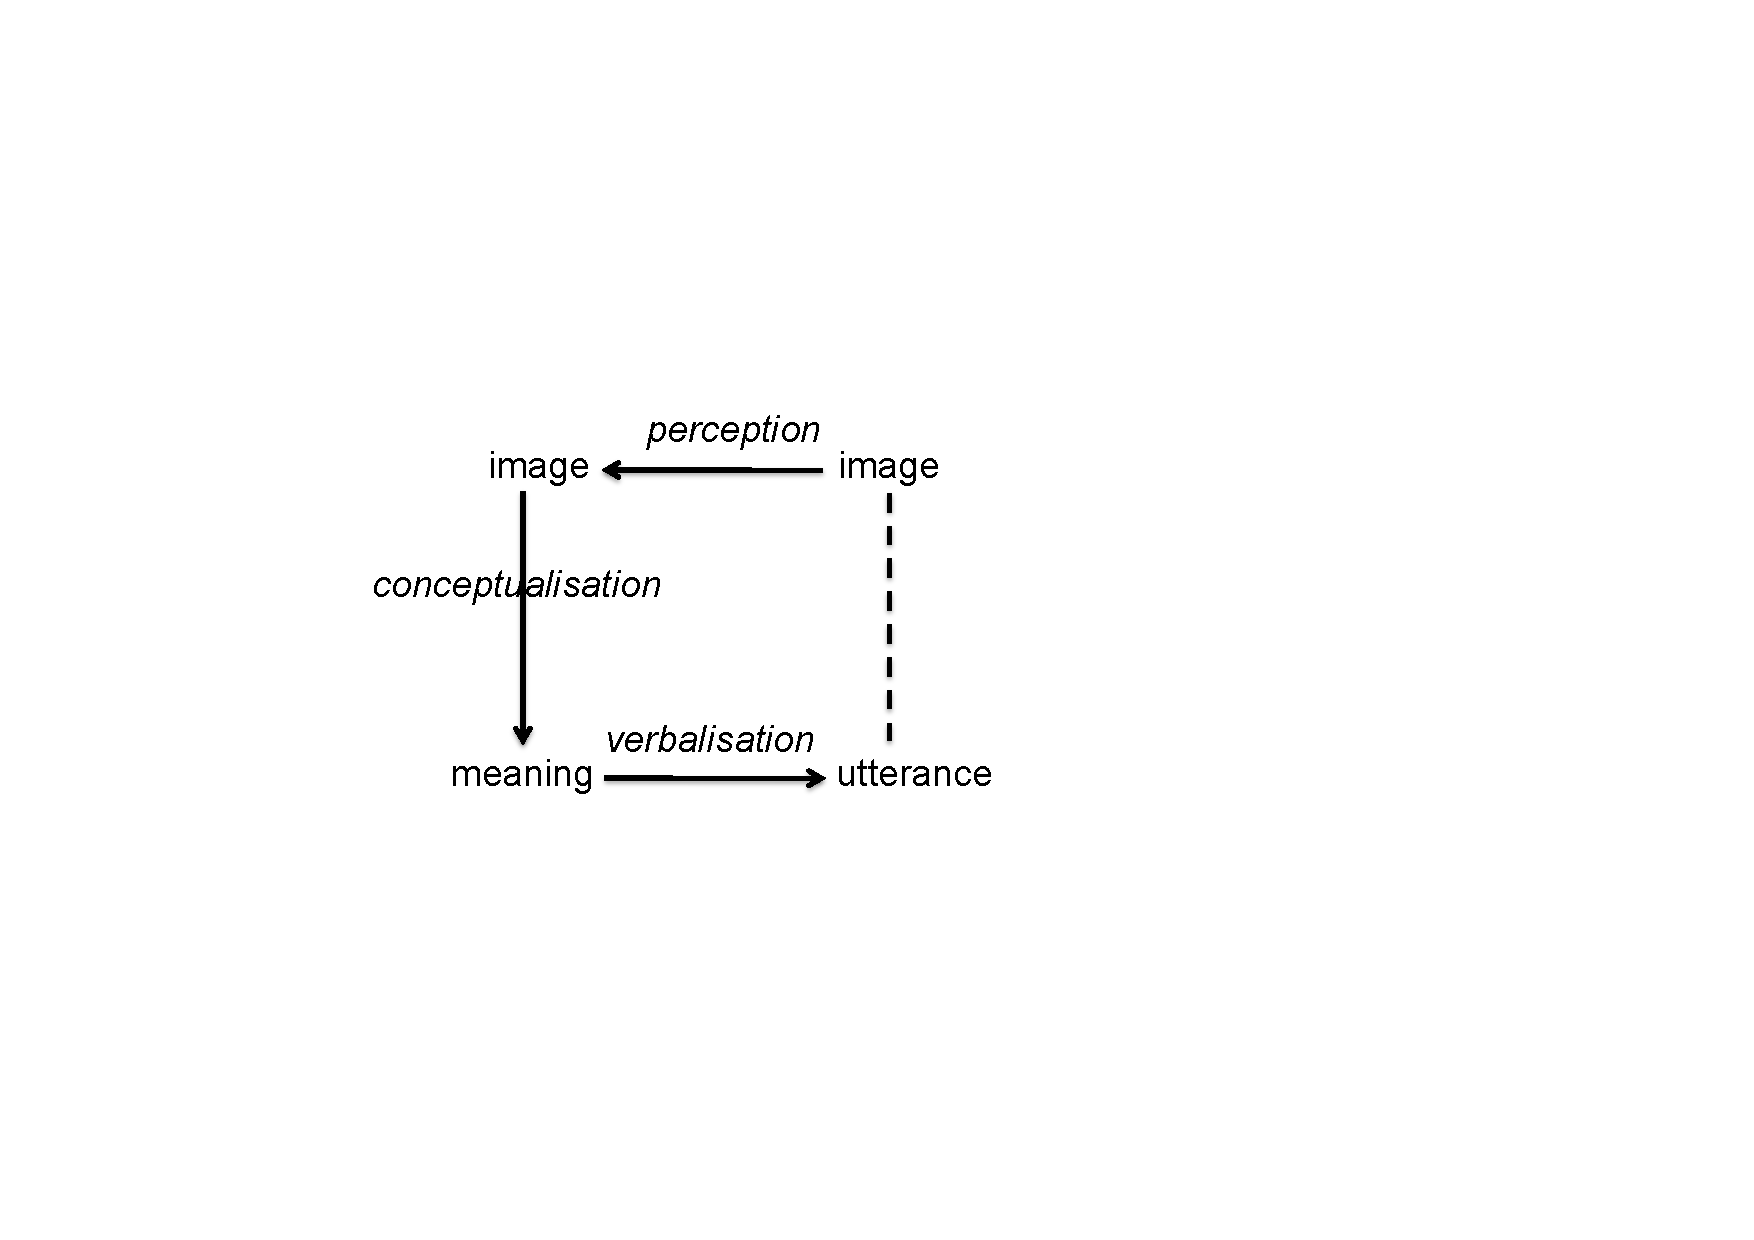
\includegraphics[width=.50\textwidth]{chap3/figs/square}}
\caption{\label{square} The general problem of 
production is broken up into three subproblems: perception, 
conceptualisation and verbalisation.}
\end{figure}

I will extensively make use of this methodology. 
This chapter has focused on perception, the next chapter focuses
exclusively on
conceptualisation, assuming that there is good segmentation and a 
decent set of sensory channels. Chapter 5 turns to the 
problem of lexicalisation, assuming that 
the agents have a shared repertoire of meanings and agree on 
what meaning to use in a particular game. Chapter 6 then puts the solutions 
for conceptualisation and lexicalisation together by coupling their
inputs and outputs and establishing the appropriate feedback connections. 
Chapter 7 then couples this system to the perceptual processes discussed
in this chapter, so that we get back to our 
original goal: understand how perceptually grounded language communication 
is possible. 

The methodology of breaking a problem into its subproblems goes quite 
a distance, but is not without danger. The processes relating
perception to language cannot be modular for reasons already mentioned. 
Each layer receives inputs which are not completely reliable and 
generates a set of possible suggestions rather than a single
`correct' solution. Constraints have to flow
from top to bottom because there is simply not enough reliable 
information to solve the problem with a straightforward sequential 
decision process. In addition, every layer is constantly adapting 
itself to the surrounding information context. New categories 
may develop, new words need to be learned, new sensory 
channels may even emerge. So, constructing a global system is going 
to be more than simply putting together its parts. There are complex
behaviors that will only become visible when the appropriate non-modular
couplings are put in place, and this is notoriously difficult to 
do and study. 

\subsection{Idealisation and realism}

To make this problem more manageable I will 
adopt a second complementary method, widely used in
engineering. We can keep the various
aspects of the global process intact, but simplify the challenge. 
We start with extremely idealised operational circumstances
and then gradually add more and more realism, until the system is 
ready to face the real world. At every step we first establish
whether the mechanisms still work, which means in the guessing
game that communicative success moves up. If this does not happen, 
we must investigate what needs to be added or changed and perhaps
reduce the complexity again to find a new bottom ground. 
If a language system does get established, we can examine 
the limits of the process before increasing the challenge once more.
During the original research, 
we extensively used this stepwise approach, often `sliding down the 
mountain' when too much complexity was introduced too quickly so 
that we were forced to take a few steps back and tackler simpler 
challenges until we got our feet on the ground again. 

We can simplify or scale down in four dimensions. 
The first dimension is that of the agents. I 
will often start by investigating a group of only two agents, then scale up
to larger and larger groups, 
and then tackle the problem of an open-ended population in which 
new members enter and others leave. Each of these steps 
introduces additional difficulties. For example, when there are
only two agents, the risk of synonyms forming is low - as we 
will see later - because the agents only interact with each 
other and so they can rapidly see whether the other one has
a word for the same meaning. But when the population is scaled up 
it is highly likely that different subgroups invent 
different words or develop new meanings.
These variations take time to propagate until
the group settles into a coherent state. 
When there is an open-ended set of agents, the new agents
in the population must acquire a language which already 
exists, which implies that we must have demonstrated that language 
acquisition goes sufficiently fast to explain cultural 
transmission. When agents leave the community, they take some
of the knowledge of the language conventions, and so we have 
to show that the whole community might destabilise. 

Second there is the dimension of the real world and how it relates 
to perception and action.  For this book, I will in any
case only use worlds restricted to 
coloured shapes on a two-dimensional surface, thus drastically reducing
the perceptual challenges, and constrain the perceptual 
task still further by supplying the agents only with a 
limited set of sensory channels. We also performed
initially many simulations with artificial worlds (to
be explained shortly) where we could carefully control various 
parameters, such as the number of objects in a scene, their
complexity, or their variation. 

But restricting the environment 
is not enough. Other aspects of perception
can seriously disrupt language communication 
in a variety of ways and each of them can be neutralised. 
We have already seen that 
in normal circumstances, the agents 
do not share the same image of reality, which introduces 
a whole array of problems. They might consequently
segment the scene differently, the pointing might not be accurate enough
(even if they both were referring to the same object), 
the segments might have very different sensory characteristics 
(as already discussed for plate 12). We have
reduced these sources of difficulty by initially using 
only one camera, then scaling up to two cameras
in the same room, and only then scaling up to many different cameras
located all over the world. Increasing or decreasing the importance 
of saliency also helps. When only the most salient sensory 
channel is used, agents have a higher chance to guess the 
right meaning (at least if their perception converges reasonably 
well), and so they can better guess the meaning of an unknown
word or go less astray with words for which they have already
a shared meaning. So by varying the saliency, we can control the 
degree of semantic ambiguity in the agents' communications. 
Divergent perception and confusing regularities in the
environment are sources of 
polysemy in language, which the agents need to 
dampen if they want their communications to be efficient and
reliable. 

Another real world aspect that we can make more or less
complex is related to the movements of the head and the pointing. 
A hearer must be able to look in the same direction as the 
speaker, so that there is a minimum shared context. The 
hearer must be able to point to the topic guessed, 
so that the speaker can see whether the communication 
succeeded. If it did not, the speaker must be able to point 
to the topic. These physical interactions are well within
the state of the art in robotics, and there exist even 
various learning systems capable of bootstrapping this capacity
from scratch.\footnote{
This is the problem of hand-eye coordination performed
in living systems by the vestibulo-oculomotor systems. 
See: \cite{Anastacio:1989}.}

But these processes will never be completely 
reliable either. So we can increase or decrease the challenge
to the agents by making the non-verbal communication and 
coordination more or less challenging. In the experiments 
reported in this book, speaker and hearer can communicate to each 
other the direction in which they 
are looking.\footnote{
This real world interaction has been developed 
by Frederic Kaplan \cite{Kaplan:1999}.}
Because they still see a 
different image due to their physical position, the 
interaction is still partly unreliable but it is sufficiently stable 
to enable the agents to bootstrap a shared communication
system, which then in turn can help to establish 
physical coordination. 

Third, there is the cognitive apparatus of the agents
implicated in language. Here we can start with a simple 
associative memory for the lexicon 
that can only handle single words
associated with single meanings, and then scale up to 
conjunctions of meanings covered by single or
multiple words, and then still further to open-ended
complex meanings and syntax. 
Each step requires additional machinery in the agents, 
which will automatically lead to more complex linguistic
forms, but it is our experience that there is great value in
trying to understand the basic process of word 
meaning acquisition before attempting to install more 
cognitive complexity in the agents' architecture. Even for the
acquisition and propagation of single word utterances there are 
still many open-ended problems. 

A final dimension concerns the transmission and 
perception of the utterance. Here again we can scale
up or down the challenge to the agents, from full-blown 
unconstrained speech in noisy environments down to perfect direct
transmission of the language form by the 
speaker and perfect recognition by the hearer. 
Complexity along this dimension has been reduced to 
the minimum in the Talking Heads experiment. Agents 
transmit utterances directly although a speech sound
is generated so that human listeners can hear which
utterance is produced as part of a game. 

\section{The GEOM world}

\is{GEOM world}One way to perform controlled experiments 
quickly and on a large scale, consists of artificially 
generating the perceptual input to the agents. 
This has the additional advantage that we can 
simplify the situations the agents have to work in
(for example have fewer types of shapes) 
and let them start initially with a shared perception. A 
simulation world that we have used extensively 
for many simulations reported later 
is the GEOM world. 

The GEOM world generates geometric shapes similar 
to the physical figures we paste on the white board. 
Possible geometric shapes are circles, triangles, 
squares, rectangles, etc. 
We can control the complexity
of the scenes that are generated  through a few parameters, for example the 
number of minimum or maximum figures, or the possible 
repertoire of shapes. We 
ignore colour and use only different grayscale 
values. To construct a scene the computer simulation 
program chooses first a random number of 
figures. Then for each figure, a shape is 
chosen, and random values for the main 
characteristics (position, height, width, grayscale)
are set. 
\begin{figure}[htbp]
  \centerline{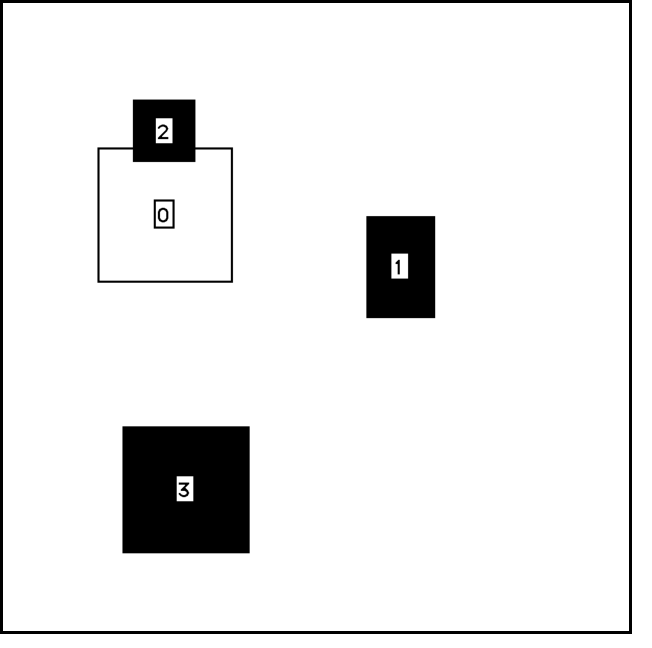
\includegraphics[width=.45\textwidth]{chap3/figs/scene9}}
\caption{\footnotesize \label{geom3} An example of the 
computer-generated scenes from the GEOM world.
Each shape is labeled for further reference.}
\end{figure}

An example of a computer-generated 
scene containing only rectangles is shown in 
\figref{geom3} (another one 
was shown earlier in \figref{rect1b}).
Given such a scene, each agent calculates
the bounding box and the segment-characteristics
for every computer-generated figure.
For the scene in \figref{geom}, which contains three
squares and a rectangle, the values of the channels
are summarised in \tabref{tab:t-geom}. 
\begin{table}
\begin{center}
\begin{tabular}{  l   l   l   l   l   l   l   l  }
\lsptoprule
 & {\itshape HPOS} & {\itshape VPOS} & {\itshape HEIGHT} & {\itshape WIDTH} & {\itshape GRAY} & {\itshape RATIO}  & {\itshape AREA} \\ \midrule
0 & 116 & 166 & 293 & 293 & 0.777 & 1.0 & 85849 \\ 
1 & 692 & 317 & 148 & 224 & 0.449 & 1.0 & 33152 \\ 
2 & 192 & 64 & 137 & 137 & 0.408 & 1.0 & 18769 \\ 
3 & 167 & 770 & 277 & 277 & 0.201 & 1.0 & 76729 \\ 
\lspbottomrule
\end{tabular}
\end{center}
\caption{\label{tab:t-geom} Sensory data for the scene shown in \figref{geom3}.}
\end{table}

After sensory-scaling we get \tabref{tab:t-geomscaled}. 
\begin{table}
\begin{center}
\begin{tabular}{  l   l   l   l   l   l   l   l  }
\lsptoprule
& {\itshape HPOS} & {\itshape VPOS} & {\itshape HEIGHT} & {\itshape WIDTH} & {\itshape GRAY} & {\itshape RATIO}  & {\itshape AREA} \\ \midrule
0 & 0.09 & 0.13 &  0.64 &  0.64 &  0.78 &  1.0 & 0.95 \\ 
1 & 0.55 & 0.25 & 0.16 & 0.41 & 0.45 & 1.0 & 0.37 \\ 
2 & 0.15 & 0.05 & 0.12 & 0.12 & 0.41 & 1.0 & 0.21 \\ 
3 & 0.13 & 0.62 & 0.59 & 0.59 & 0.20 & 1.0 & 0.85 \\ 
\lspbottomrule
\end{tabular}
\end{center}
\caption{\label{tab:t-geomscaled} Sensory data after scaling for the scene shown in \figref{geom3}.}
\end{table}

The output of the simulation is exactly the same as the one from real vision 
so that we can easily switch between simulation 
and physical experimentation. 

\subsection{Simulation versus experimentation}

Working with simulations has obvious advantages for 
speeding up development and systematic testing, 
but it does not replace experimentation with 
physical robots. It is true that 
building an experimental apparatus such as we built
for the Talking Heads experiment is a very 
non-trivial engineering project, particularly because 
of the teleporting infrastructure that enables the agents 
to travel to multiple sites and thus 
experience different physical environments or the same 
environment from different points of view. 
One might therefore wonder why we have persisted
to go to such great length in constructing
a real-world physical infrastructure. Why are
experiments with robotic agents necessary or 
desirable? Is it not enough to conduct simulation
experiments given that they can be done so much 
more easily? 

Computer simulations calculate the consequences of a
theoretical model. For example, we can implement Newton's
model of the solar system and simulate the movements
of the planets around the sun by calculating for 
small time steps the position of each planet and hence
the trajectories they follow. All the aspects of 
a calculation are under the scientist's control and it 
is therefore possible to use this method to examine whether a theory can 
be operationalised, whether it is coherent, and whether 
it is complete, i.e. whether it covers all 
aspects of the phenomena one tries to understand. 
Simulations can be inspected, re-executed
or reprogrammed by anyone who cares to challenge them and
other researchers can try to achieve the
same performance with alternative approaches, so that 
different theories can be compared in an objective way. 

Computer simulations can be set up for any theory which 
is formalisable, and hence for theories of cognition
and language as well. We need to implement the cognitive architecture
of the agent and then examine what happens when the agent
engages in interactions, i.e. when data is supplied from 
real or simulated scenes. Computer simulations of cognitive mechanisms
provide proof that they can be instantiated
on physical systems, even though it may still be
a mystery how the brain, 
itself a physical system, implements similar mechanisms. 
Computational simulation is of course 
not restricted to the theories I put forward in 
this book. Any theory claiming
to explain the origins of language and meaning 
should be testable by computer simulation, so that 
it is clear what form the architecture takes and whether
it does the job. All this is a big step compared to 
the early days of cognitive modelling when one was
supposed to believe on faith whether a certain cognitive
architecture could be instantiated by a physical 
system and whether it was indeed able to exhibit the functionality 
that was ascribed to it. 

But computer simulations have two major shortcomings, 
which makes them only one of the tools in the toolkit 
of the cognitive scientist. First of all, computer simulations by
themselves do not empirically validate a theory. When 
a computer screen shows pictures of planets moving around 
the sun, there is nothing that says that this is also 
the way the planets move. To validate the theory, large amounts of
data need to be collected of
the natural phenomena, and the simulation 
results have to be compared with the real world data to determine a sufficient
fit. In this book, we are primarily concerned with 
formulating new plausible models for cognition and particularly
for the origins of cognition, not yet with their
empirical validation; this exciting work is left for the future. 

However, there is a second shortcoming. Cognitive systems
must deal with the real physical world in its infinite variety 
and complexity. If we perform only computer simulations, 
we not only model the cognitive mechanisms of the 
agents but also the environments which they are 
confronted with. We validate the model only with 
respect to stylised worlds. Of course we can make
such worlds much more sophisticated, but 
there is never a guarantee that they are going to be
representative of the real worlds that
embodied cognitive agents have to deal with. 
The more realistic computer simulations 
become, that is the more aspects of reality they reliably 
take into account, the more the simulation starts to approach 
reality and the more a simulation may tell us whether
the proposed mechanisms live up to realistic circumstances.
But there will always be a huge difference between 
computer-simulated worlds and real worlds, as any
roboticist knows all too well. 
And this is why we need to do experiments
with physical robots and real-world environments. 

Of course, it is useful and efficient to 
conduct simulations as part of the discovery process 
but true validation of a cognitive architecture 
can only come when 
the system is confronted with a real physical environment. 
It forces us to attack the final known or hidden 
assumptions in the theory's operational validation. It
forces us to address the issue of sensing, using
real world physical sensors. Therefore, an experiment 
like the Talking Heads experiment has
a much greater force in 
convincing the sceptic. It is like testing the design 
for an airplane by building and flying one, as opposed
to demonstrating the idea only in simulation. 

\section{Conclusions}

This chapter focused on the perceptual layer which 
is responsible for interfacing the external physical 
world with the internal world of the agents. The 
interface is based on sensors to transduce external states
into internal states and actuators to transduce internal states into
external states. Four sorts of operations take place 
on raw sensory data making them more amenable to 
categorisation, conceptualisation and consequently 
language communication: Features in the 
form of micro-structures are extracted, the image is 
segmented in coherent units using region growing or 
countour finding, segment characteristics such as 
average colour or size are derived, and characteristics 
are transformed or scaled to bring out salient 
features and aid to achieve categorial constancy. 

The Talking Heads use 
standard techniques from computer vision research. Research
in this field is indeed so advanced that a large number 
of algorithms for segmenting images and extracting information about
image segments could be taken "off the shelf" and re-programmed to get 
a vision system that is adequate for the task setting 
of the Talking Heads experiment. This will, of course, no 
longer be the case if the environment is made more challenging
and more open to novel situations. Very quickly we would 
then reach the limits of what can currently be done using
standard techniques. Nevertheless for our purpose of 
exploring language and meaning, the Talking Heads 
vision system gives 
a sufficiently rich and reliable segmentation and 
characterisation of the scene so that an investigation
of how real world scenes might be conceptualised and 
verbalised, has become possible. 
